\newcommand{\slot}[2]{%
  \lstindex{#1} & #2 \\\hline%
}%

\newcommand{\optSlot}[2]{%
  \textcolor{gray}{[\lstindex{#1}]} & #2 \\\hline%
}%

\newenvironment{slots}[1][Slots]
{%
  \subparagraph{#1}%
  \begin{flushleft}%
    \tablehead{}%
    \begin{supertabular}{|m{2.8669999cm}|m{12.472cm}|}%
      \hline%
      \textbf{Slot} &%
      \textbf{Description}\\\hline%
    }
    {%
    \end{supertabular}%
  \end{flushleft}%
}

\newcommand{\refFacet}[2][]%
  {\hyperref[sec:facet:#2]{\lstinline|#2|#1 (\autoref*{sec:facet:#2})}}

\newcommand{\facet}[2][]{%
  \ifthenelse{\equal{#1}{}}{%
    \subsection{#2\index{#2@\lstinline{#2}}}%
  }{%
    \subsection{#2 (subclass of #1)\index{#2@\lstinline{#2}}}%
  }%
  \label{sec:facet:#2}
}


\chapter{\urbi Ready™-Certification Standard}
\label{sec:naming}

\begin{center}
  
\includegraphics[scale=.5]{img/urbi-ready}
\end{center}

% \section{Introduction}

This section aims at clarifying the naming conventions in \urbi
Engines for standard hardware/software devices and components
implemented as UObject and the corresponding methods/attributes/events
to access them. The list of available hardware types and software
component is increasing and this document will be updated
accordingly. Please contact us directly, should you be working on a
component not described or closely related to one described here:

\begin{center}
  \email{standard@gostai.com}
\end{center}

Any implementation of an \urbi server must comply with the latest
version of this standard to get the ``\urbi ready'' certification from
Gostai S.A.S.


Gostai S.A.S. is currently the only authority which has the ability to
deliver an ``\urbi Ready'' certification.

``\urbi Ready'' and the associated logo are trademarks of Gostai
S.A.S. and should not be used or displayed in any way without an
explicit written agreement from Gostai.

\section{The Structure Tree}

The robot will be described as a set of \textit{components} organized
in a hierarchical structure called the \textit{structure tree}. The
relationship between a component and a sub-component in the tree is a
‘part-of’ inclusion relationship. From the point of view of \urbi,
each component in the tree is an object, and it contains attributes
pointing to its sub-components. Here is a example illustrating a part
of a hierarchy that could be found with a humanoid robot:

\begin{center}
  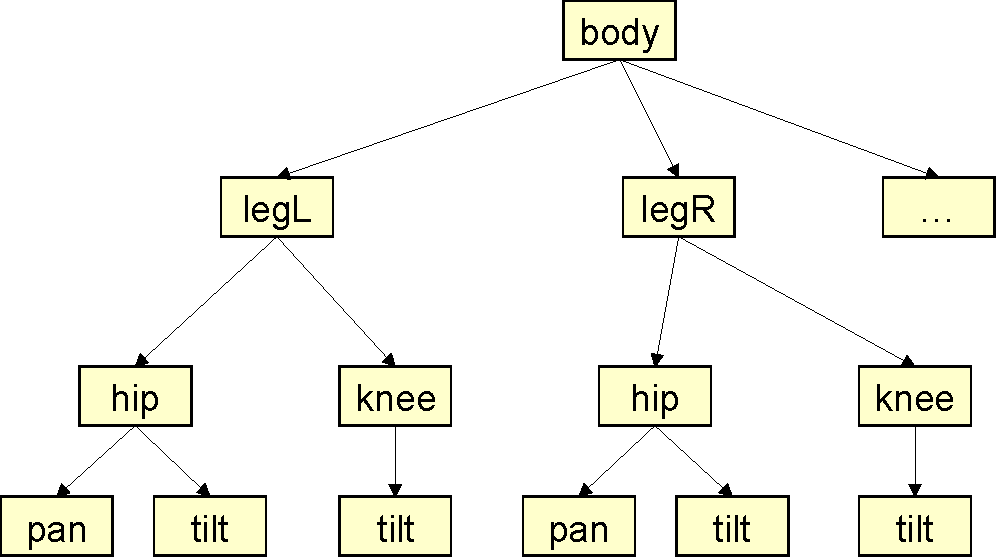
\includegraphics[width=.8\linewidth]{img/structure-tree}
\end{center}

The leaves of the tree are called \textit{devices}, and they usually
match physical devices in the robot: motors, sensors, lights, camera,
etc. Inside \urbi, the various objects corresponding to the tree
components are accessed by following the path of objects inclusions,
like in the example below (shortcuts will be described later):

\begin{urbifixme}
body.legR.hip.tilt;
body.legL.knee.led;
body.legL.hip;
// ...
\end{urbifixme}


The structure tree should not be mistaken for a representation of the
kinematics chain of the robot. The kinematics chain is built from a
subset of the devices corresponding to motor devices, and it
represents spatial connections between them. Except for these motor
devices, the structure tree components do not have a direct
counterpart in the kinematics chain, or, if they do, it is as a subset
of the kinematics chain (for example, \texttt{legR} is a subset of the
whole kinematics chain).


The goal of this standard is to provide guidelines on how to define
the components and the structure tree, knowing the kinematics chain of
the robot.

\section{Frame of Reference}

In many cases, it will be necessary to refer to an absolute frame of
reference attached to the robot body. To avoid ambiguities, the
standard frame of reference will have the following definition:

\begin{center}
  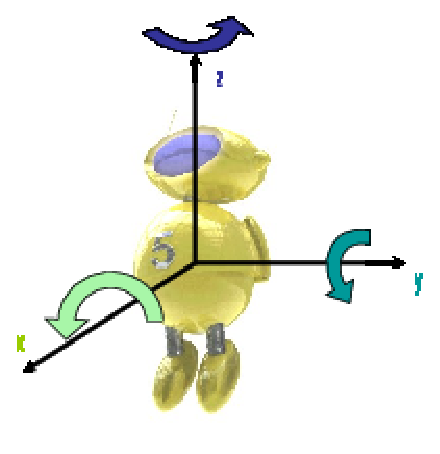
\includegraphics{img/reference-frame}
\end{center}

\begin{description}
\item[Origin] the center of mass of the robot
\item[X axis] oriented towards the front of the robot. If there is a
  camera, the front is defined by the default direction of the camera,
  otherwise the front will be seen as the natural frontal orientation
  for a mobile robot (the direction of “forward” movement). If the
  robot is not naturally oriented, the X axis will be chosen to match
  the main axis of symmetry of the robot body and it will be oriented
  towards the smallest side, typically the top of a cone for
  example. In case of a perfectly symmetrical body, the X axis can be
  chosen arbitrarily but a clear mark should be made visible on the
  robot body to indicate it.
\item[Z axis] oriented in the opposite direction from the gravity. If
  there is no gravity or natural up/down orientation in the
  environment or normal operation mode of the robot, the Z axis should
  be chosen in the direction of the main axis of symmetry in the
  orthogonal plane defined by the X axis, oriented towards the
  smallest side. In case of a perfectly symmetrical plane, the Z axis
  can be chosen arbitrarily but a clear mark should be made visible on
  the robot body to indicate it.
\item[Y axis] oriented to make a right-handed coordinate system.
\end{description}


The axes are oriented in a counter-clockwise direction, as depicted in
the illustration above.

\section{Component naming}

The name of a component A, which is a sub-component of component B, is
divided into two parts: the generic designation of a subpart of the
kinematics chain (like ‘leg’, ‘head’, ‘finger’) that A is referring
to, and optionally some topological disambiguator relative to its
position within the component B it belongs to. For example, when there
are two legs, we need to differentiate between the right and left leg,
relative to the body component they belong to. The first part is
called the \textit{designation}, and the second optional part is
called the \textit{localization}.

\paragraph{Designation}


The designation of a component is a usually robot-specific and depends
on the class of the robot (wheeled, humanoid, animaloid, etc). We will
give in the following chapters some guidelines for the most current
designations, and we will give more advanced rules for rare customized
cases.


The designation is the critical part of the naming standard. We cannot
possibly cover all future configurations and conceivable robot complex
bodies, but the current document will grow whenever we find a new
case.  We hope to be already covering most of the main cases you can
find in the industry.

\paragraph{Localization}

Localization is necessary when there are two identical sub-components
A1 and A2 belonging to the same component B, like for example two legs
or two arms attached to the main body. Usually this can be sorted out
with simple geometric qualifiers like \textit{Right/Center/Left},
\textit{Front/Middle/Back} or \textit{Up/In-between/Down}. The naming
convention is to use the first letter of the geometric characteristic,
like R for Right, I for In-between.  Note that “right” or “front” are
understood here from the point of view of a man standing and looking
in the direction of the X-axis of the robot, and \textit{Up/Down}
matches the Z-axis, as depicted in the figure below:

\begin{center}
  
\includegraphics[width=.5\linewidth]{img/cube}
\end{center}

Several geometric qualifiers can be used at the same time to further
refine the position. As a convention, side information comes first
(R/C/L), followed by the depth information (F/M/H) and then the height
information (U/I/D).

You can further qualify a side+depth localization with an additional
R/L side information. This can be used in the typical layout below:

\begin{center}
  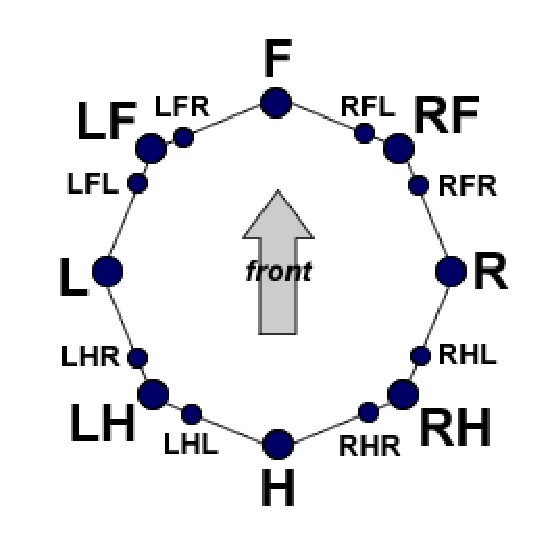
\includegraphics{img/lrfh}
\end{center}

This dual positioning using side+depth can also be used to combine
side+height or height+depth information.

Some layouts will typically imply a bilateral organization like for
example an insectoid robot with a series of 3 legs on both side of its
body. In that case, an array will be used and follow the geometrical
localization (R/L). The smaller the number, the closer to the front:
R[1], R[2], R[3] and L[1], L[2], L[3]. This can be used when there is
at least 3 components on each side, otherwise the
\textit{Front}/\textit{Back} approach prevails.

Some components like spines or tails are highly articulated with a set
of identical sub-components. When talking about these sub-components,
the above localization should be replaced by an array with a numbering
starting at 0. The smaller the number, the closer the sub-component is
to the robot main body. For surface-like sub-components, like skin
touch sensors, the array can be two dimensional.

Other possible localization for sensors are the X, Y and Z axis
themselves, like for example for an accelerometer or a gyro sensor,
available in each of the three directions.


Examples of component names including localization:

\begin{urbifixme}
legR, legL, armR, armL;
fingerR, fingerC, fingerL;      // three fingers hand
joint[0], joint[1] ... joint[5] // from tail
touch[478][124]                 // from skin
accelX, accelY, accelZ;         // typical accelerometer
gyroX, gyroY, gyroZ;            // typical gyro sensor
\end{urbifixme}

\section{Facets}

\urbi allows multiple inheritances between objects. This feature can be
used to introduce the notion of “facet”. A facet is an object in \urbi
that describes some aspect of a type of component.

For example, for a joint, we can have a “swivel” facet, used to define
patella joints. For the robot body itself, we have a “mobile” facet
describing mobile robots, which includes some standard way of
requesting a move forward, a turn, etc. A robot with a Pan/Tilt camera
or otherwise moving camera will have the “panoramic” facet which is
abstracting the way the robot can turn its gaze in any direction.

In short, facets are standard Urbi objects that components can inherit
from to acquire some functionalities, expressed as a standard
interface. We will describe in the following pages a few of the most
standard facets. Each facet should be reimplemented for any particular
robot that uses them, for example the “mobile” facet will have a
completely different implementation with a humanoid robot and a wheeled
robot.

\facet{identity}

Contains information about the robot identity.

\begin{slots}
  \slot{type}
  {
    This describes the robot category among: humanoid, fourlegged,
    wheeled, industrial arm. It gives a general idea of the robot
    family, but does not replace a more systematic probe of available
    services by investigating the list of attributes of the object.
  }

  \slot{name}%
  {%
    Name of the robot.%
  }

  \slot{model}%
  {%
    Model of the robot.%
  }

  \slot{serial}%
  {%
    Serial number (if available).%
  }

\end{slots}


\facet{network}

Contains information about the network identification of the robot.

\begin{slots}
  \slot{IP}%
  {%
    IP address of the robot.%
  }

  \slot{gateway}%
  {%
    Gateway IP address.%
  }

  \slot{latency}%
  {%
    Measured average network latency.%
  }

  \slot{bandwidth}%
  {%
    Measured average network bandwidth.%
  }

\end{slots}

\facet{motor}

This facet is used to describe a generic motor controller.

\begin{slots}
  \slot{val}%
  {%
    This slot is a generic pointer to a more specific slot describing
    the motor position, like \texttt{position} or \texttt{angle},
    depending on the type of motor. It is mandatory in the Urbi Ready
    standard as a universal proxy to control an actuator. The more
    specific slot is described in a subclass of \texttt{motor}.%
  }

  \slot{PGain}%
  {%
    Controls the P gain of the PID controller.%
  }

  \slot{IGain}%
  {%
    Controls the I gain of the PID controller.%
  }

  \slot{DGain}%
  {%
    Controls the D gain of the PID controller.%
  }

\end{slots}

\facet[motor]{linearMotor}


This facet is used to describe a linear motor controller.

\begin{slots}
  \slot{position}%
  {%
    Position of the motor in centimeters.  Pointed to by the
    \texttt{val} slot.%
  }

  \slot{force}%
  {%
    Intensity of the measured or estimated force applied on a linear
    motor.%
  }

\end{slots}

\facet[motor]{rotationalMotor}


This facet is used to describe a rotational motor controller.

\begin{slots}
  \slot{angle}%
  {%
    Angle of the motor in degree, modulo 360. Pointed to by the
    \texttt{val} slot.%
  }

  \slot{turn}%
  {%
    Absolute angular position of the motor, expressed in number of
    turns.%
  }

  \slot{torque}%
  {%
    Intensity of the measured or estimated torque applied on the
    motor.%
  }

\end{slots}


\facet{sensor}

This facet is used to describe a generic sensor.

\begin{slots}
  \slot{val}%
  {%
    This slot is a generic pointer to a more specific slot describing
    the sensor value, like \texttt{distance} or \texttt{temperature},
    depending on the type of sensor. It is mandatory in the Urbi Ready
    standard as a universal proxy to read a sensor. The more specific
    slot is described in a subclass of \texttt{sensor}.%
  }

\end{slots}


\facet[sensor]{distanceSensor}

This facet is used to describe a distance sensor (infrared, laser,
ultrasonic...).

\begin{slots}
  \slot{distance}%
  {%
    Measured distance expressed in meters.  Pointed to by the
    \texttt{val} slot.%
  }

\end{slots}


\facet[sensor]{touchSensor}

This facet is used to describe a touch pressure sensor (contact,
induction,...).

\begin{slots}
  \slot{pressure}%
  {%
    Intensity of the pressure put on the touch sensor. Can be 0/1 for
    simple buttons or expressed in Pascal units. Pointed to by the
    \texttt{val} slot.%
  }

\end{slots}


\facet[sensor]{accelerationSensor}

This facet is used to describe an accelerometer.

\begin{slots}
  \slot{acceleration}%
  {%
    Acceleration expressed in m/s2.  Pointed to by the \texttt{val}
    slot.%
  }

\end{slots}

\facet[sensor]{gyroSensor}
This facet is used to describe an gyrometer.

\begin{slots}
  \slot{acceleration}%
  {%
    Acceleration expressed in rad/s2.  Pointed to by the \texttt{val}
    slot.%
  }
\end{slots}

\facet[sensor]{temperatureSensor}
This facet is used to describe a temperature sensor.

\begin{slots}
  \slot{temperature}%
  {%
    Measured temperature in Celsius degrees.  Pointed to by the
    \texttt{val} slot.%
  }

\end{slots}

\facet{mobile}

Mobile robots all share this generic interface to provide high order
level motion control capabilities.

\begin{slots}
  \slot{go(x)}%
  {%
    Move approximatively x meters forward if x is positive, backward
    otherwise.%
  }

  \slot{turn(x)}%
  {%
    Turn right approximatively x degrees.  x can be a positive or
    negative value.%
  }

\end{slots}

\facet{tracker}

Camera-equipped robots can sometimes move the orientation of the field
of view horizontally and vertically, which is a very important feature
for many applications. In that case, this facet abstracts how such
motion can be achieved, whether it is done with a pan/tilt camera or
with whole body motion or a combination of both.

\begin{slots}
  \slot{yaw}%
  {%
    Rotational articulation around the Z axis in the robot, expressed
    in degrees.%
  }

  \slot{pitch}%
  {%
    Rotational articulation around the Y axis in the robot, expressed
    in degrees.%
  }

\end{slots}

\facet{videoin}

The videoin facet groups every information relative to cameras or any
image sensor.

\begin{slots}
  \slot{val}%
  {%
    Binary value corresponding to the image, expressed in the current
    unit (RGB, jpeg, YCrCb...). The unit can be changed like any other
    regular unit in Urbi. %
  }

  \slot{xfov}%
  {%
    The x Field Of View of the camera expressed in degrees.%
  }

  \slot{yfov}%
  {%
    The y Field Of View of the camera expressed in degrees.%
  }

  \slot{height}%
  {%
    Height of the image in the current resolution, expressed in
    pixels%
  }

  \slot{width}%
  {%
    Width of the image in the current resolution, expressed in pixels%
  }

  \slot{shutter}%
  {%
    The shutter speed (expressed in ms). 0 if non applicable.%
  }

  \slot{wb}%
  {%
    White balance (expressed with an integer value depending on the
    camera documentation). 0 if non applicable.%
  }

  \slot{gain}%
  {%
    Camera gain amplification (expressed as a coefficient between 0
    and infinity). 1 if non applicable.%
  }

  \slot{resolution}%
  {%
    Can be used to specify a given resolution, expressed as a
    percentage of the maximal resolution of the camera (number between
    0 and 1). 1 if non applicable.

    Once modified, the effective resolution in X/Y can be checked with
    the width and height slots.%
  }

\end{slots}

\facet{audioout}
The audioout facet groups every information relative to speakers.

\begin{slots}
  \slot{val}%
  {%
    The speaker value, expressed as a binary, in the format given by
    the binary header during the assignment.

    Speakers are write-only devices, so there is not much sense in
    reading the content of this attribute. At best, it returns the
    remaining sound to be played if it is not over yet, but this is
    not a requirement.%
  }

  \slot{remain}%
  {%
    The amount of time remaining to play in the speaker sound buffer
    (expressed in \textit{ms} as a default unit).%
  }

  \slot{playing}%
  {%
    This is a boolean value which is true when there is a sound
    currently playing (the buffer is not empty)%
  }

  \slot{volume}%
  {%
    Volume of the play back, in decibels.%
  }
\end{slots}



\facet{audioin}

The audioin facet groups every information relative to microphones.

\begin{slots}
  \slot{val}%
  {%
    Binary value corresponding to the sound heard, expressed in the
    current unit (wav, mp3...). The unit can be changed like any other
    regular unit in Urbi.

    The content is the sound heard by the microphone since the last
    update event.%
  }

  \slot{duration}%
  {%
    Amount of sound in the val attribute, expressed in \textit{ms}.%
  }

  \slot{gain}%
  {%
    Microphone gain amplification (expressed between 0 and 1)%
  }
\end{slots}


\facet{blobDetector}

Ball detectors, marker detectors and various feature-based detectors
should all share a similar interface. They extract a part of the image
that fits some criteria and define a “blob” accordingly. Here are the
typical slots expected:

\begin{slots}
  \slot{x}%
  {%
    The x position of the center of the blob in the image%
  }

  \slot{y}%
  {%
    The y position of the center of the blob in the image%
  }

  \slot{ratio}%
  {%
    The size of the blob expressed as a normalized image size: 1 =
    full image, 0 = nothing.%
  }

  \slot{visible}%
  {%
    A Boolean expressing whether there is a blob in the image or not
    (see threshold)%
  }

  \slot{threshold}%
  {%
    The minimum value of ratio to decide that the blob is visible.%
  }

  \slot{orientation}%
  {%
    Angle of the main ellipsoid axis of the blog (0 = horizontal),
    expressed in degrees.%
  }

  \slot{elongation}%
  {%
    Ratio between the main and the second diameter of the blob
    enveloping ellipse.%
  }

\end{slots}

\facet{textToSpeech}
Text to speech allows to read text using a speech synthetizor. Default
implementations should use the \texttt{speaker} component (or alias) as
their default sound output.

\begin{slots}
  \slot{lang}%
  {%
    The language used, in international notation (fr, en, it…): ISO
    639%
  }

  \slot{speed}%
  {%
    How fast the voice should go, between 0 and 1.%
  }

  \slot{pitch}%
  {%
    Voice pitch, between 0 and 1.%
  }

  \slot{gender}%
  {%
    Gender of the speaker (0:male/1:female)%
  }

  \slot{age}%
  {%
    Age of the speaker, if applicable%
  }

  \slot{name}%
  {%
    Most TTS engine will propose several voices, this attributes
    allows picking one. It’s a string identifier specific to the TTS
    developer.%
  }

  \slot{say(s)}%
  {%
    Speak the sentence given in parameter \var{s}.%
  }

  \slot{voicexml(s)}%
  {%
    Speak the text \var{s} expressed as a VoiceXML string.%
  }

  \slot{script(s)}%
  {%
    Speak the text \var{s} augmented by script markups (see specific
    Gostai documentation) to generate \urbi events.%
  }

\end{slots}


\facet{speechRecognizer}

Speech recognition allows to transform a stream of sound into a text
using various speech recognition algorithms. Default implementations
should use the \texttt{micro} component (or alias) as their default
sound input.

\begin{slots}
  \slot{lang}%
  {%
    The language used, in international notation (fr, en, it…): ISO
    639%
  }
\end{slots}

\begin{slots}[Events]
  \slot{hear(s)}%
  {%
    This event has one parameter which is the string describing what
    the speech engine has recognized (can be a word or a sentence).%
  }
\end{slots}

\section{Standard Components}

Standard components correspond to components typically found in wheeled
robots, humanoid or animaloid robots, or in industrial arms.


The table on the next pages summarize the currently referenced standard
components, with a description of potential components that they could
be subcomponent of, a description of potential components they may
contain, and a list of relevant facets. This table should be seen as a
quick reference guide to identify available components in a given
robot.

\paragraph{Yaw/Pitch/Roll orientation: guideline}

It is not always clear which rotational direction corresponds to the
yaw, pitch or roll components (listed in the table below). This is a
quick guideline to help determine the proper association.

Let us consider the robot in its resting, most prototypical position,
like “standing” on two or four legs for a humanoid or animaloid, and
let all members “naturally” fall under gravity. When gravity has no
effect on a certain joint (because it is in the orthogonal plan to Z,
for example), the medium position between rangemin and rangemax should
be used. The body position achieved will be considered as a reference.
Then for each component that is described in terms of yaw/pitch/roll
sub-decomposition, the association will be as follow:

\begin{description}
\item[yaw] rotational articulation around the Z axis in the robot.
\item[pitch] rotational articulation around the Y axis in the robot.
\item[roll] rotational articulation around the X axis in the robot.
\end{description}

When there is no exact match with the X/Y/Z axis, the closest match, or
the default remaining available axis, should be selected to determine
the yaw/pitch/roll meaning.

\bigskip

\newcommand{\component}[5]
{
  \lstindex{#1} &
  #5 &
  \code{#2} &
  \code{#3} &
  \code{#4}\\\hline
}

\tablehead{\hline
\textbf{Name} &
\textbf{Description} &
\textbf{Sub. of} &
\textbf{Contains} &
\textbf{Facets} \\\hline}
\begin{supertabular}{|m{.115\linewidth}|m{.45\linewidth}|*{4}{m{.12\linewidth}|}}
  \component{robot}{-}{body}{identity network mobile tracker}{
    %%
    This is the main component that represents an abstraction of the
    robot.
    %%
  }

  \component{body}{robot}{arm leg neck head wheel tail skin torso
    \ldots}{-}{
    %%
    This is the main component that contains every piece of hardware
    in the robot. This includes all primary kinematics sub-chains
    (arms, legs, neck, head, etc) and non-localized sensor arrays,
    typically body skin or heat detectors.  Localized sensors, like
    fingertips touch sensors, will typically be found attached to the
    finger component they belong and not directly to the body.
    %%
  }

  \component{leg}{body}{hip knee ankle foot joint}{-}{
    %%
    Legs are found in humanoid or animaloid robots and correspond to
    part of the kinematics chain that are attached to the main body by
    one extremity only and which do touch the ground in normal
    operation mode (unlike arms). A typical configuration for
    humanoids contains a hip, a knee and an ankle. If the leg is more
    segmented, the leg can be described with a simple array of joints.
    %%
  }

  \component{arm}{body}{shoulder elbow wrist hand grip  joint}{-}{
    %%
    Unlike legs, an arm’s extremity does not always touch the ground
    in normal operating mode. This applies to humanoid robots or
    single-arm industrial robots. Arms supersede legs in the
    nomenclature: if a body part behaves alternatively like an arm and
    like a leg, it will be considered as an arm.
    %%
  }

  \component{shoulder}{arm}{yaw pitch roll}{-}{
    %%
    The shoulder is the upper part of the arm. It can have one, two or
    three degrees of freedom and is the closest part of the arm
    relative to the body.
    %%
  }

  \component{elbow}{arm}{pitch}{-}{
    %%
    Separates the upper arm and the lower arm, this is usually a
    single rotational axis.
    %%
  }

  \component{wrist}{arm}{yaw pitch roll}{-}{
    %%
    Connects the hand and the lower part of the arm. Usually three
    degrees of freedom axis.
    %%
  }

  \component{hand}{arm}{finger}{-}{
    %%
    The hand is an extension of the arm that usually holds
    fingers. It’s not the wrist, which is articulated and between the
    arm and the hand.
    %%
  }

  \component{finger}{hand}{touch}{motor}{
    %%
    Fingers are a series of articulated motors at the extremity of the
    arm, and connected to the hand. They are usually localized with
    arrays and/or lateral localization respective to the hand.
    %%
  }

  \component{grip}{arm hand}{touch}{motor}{
    %%
    Simple two-fingers system.
    %%
  }

  \component{hip}{leg}{yaw pitch roll}{-}{
    %%
    The hip is the upper part of the leg and connects it to the main
    body. It can have one, two or three degrees of freedom.
    %%
  }

  \component{knee}{leg}{pitch}{-}{
    %%
    Separates the upper leg and the lower leg, this is usually a
    single rotational axis.
    %%
    }

  \component{ankle}{leg}{yaw pitch roll}{-}{
    %%
    Connects the foot and the lower part of the leg. Usually three
    degrees of freedom axis.
    %%
    }

  \component{foot}{leg}{touch}{-}{
    %%
    The foot is an extension of the leg that usually holds toes. It’s
    not the ankle, which is articulated and between the leg and the
    foot. The foot can also contain touch sensors in simple
    configurations.
    %%
  }

  \component{toe}{foot}{touch}{motor}{
    %%
    Like fingers, but attached to the foot.
    %%
  }

  \component{neck}{body}{yaw pitch roll}{-}{
    %%
    The neck corresponds to a degree of freedom not part of the head,
    but relative to the rigid connection between the head and the main
    body.
    %%
  }

  \component{tail}{body}{joint}{-}{
    %%
    A tail is a series of articulated motors at the back of the robot.
    %%
  }

  \component{head}{body neck}{camera mouth ear lip eye eyebrow}{-}{
    %%
    The head main pivotal axis.
    %%
  }

  \component{mouth}{head}{lip}{motor}{
    %%
    The robot mouth (open/close)
    %%
  }

  \component{ear}{head}{-}{motor}{
    %%
    Ears may have degrees of freedom in
    certain robots.
    %%
  }

  \component{joint}{tail arm leg lip}{-}{motor}{
    %%
    Generic articulation in the robot.
    %%
  }

  \component{yaw}{neck knee ankle shoulder elbow wrist
    torso}{-}{rotational\-Motor}{
    %%
    Rotational articulation around the Z axis in the
    robot. \textit{See the introduction paragraph on yaw/pitch/roll
      orientation for more details on how to identify which direction
      corresponds to yaw.}
    %%
  }

  \component{pitch}{neck knee ankle shoulder elbow wrist
    torso}{-}{rotational\-Motor}{
    %%
    Rotational articulation around the Y axis in the
    robot. \textit{See the introduction paragraph on yaw/pitch/roll
      orientation for more details on how to identify which direction
      corresponds to pitch.}
    %%
  }

  \component{roll}{neck knee ankle shoulder elbow wrist
    torso}{-}{rotational\-Motor}{
    %%
    Rotational articulation around the X axis in the
    robot. \textit{See the introduction paragraph on yaw/pitch/roll
      orientation for more details on how to identify which direction
      corresponds to roll.}
    %%
  }

  \component{lip}{mouth}{joint}{motor}{
    %%
    Corresponds to animated lips.
    %%
  }

  \component{eye}{head}{camera}{-}{
    %%
    Corresponds to the eyeball pivotal axis.
    %%
    }

  \component{eyebrow}{head}{joint}{motor}{
    %%
    Some robots will have eyebrow with generally one or several degree
    of freedom.
    %%
    }

  \component{torso}{body}{yaw pitch roll}{-}{
    %%
    This corresponds to a pivotal or rotational axis in the middle of
    the main body.
    %%
    }

  \component{spine}{torso}{joint}{-}{
    %%
    This is a more elaborated version of “torso”, with a series of
    articulations to give several degrees of freedom in the back of
    the robot.
    %%
    }

  \component{clavicle}{body}{-}{motor}{
    %%
    This is not to be mixed up with the “top of the arm” body part. It
    is an independent degree of freedom that can be used to bring the
    two arms closer in a sort of “shoulder raising” movement.
    %%
    }

  \component{touch}{finger grip foot toe}{-}{touchSensor}{
    %%
      Touch sensor.
    %%
    }

  \component{gyro}{body}{-}{gyroSensor}{
    %%
      Gyrometer sensor.
    %%
    }

  \component{accel}{body}{-}{accel\-eration\-Sensor}{
    %%
      Accelerometer sensor.
    %%
    }

  \component{camera}{head body}{-}{videoin}{
    %%
    Camera sensor. If several cameras are available, localization
    shall apply, however there must always be an alias from
    \texttt{camera} to one of the effective camera (like
    \texttt{cameraR} or \texttt{cameraL}).
    %%
    }

  \component{speaker}{head body}{-}{audioin}{
    %%
    Speaker device. If several speakers are available, localization
    shall apply, however there must always be an alias from
    \texttt{speaker} to one of the effective speakers (like
    \texttt{speakerR} or \texttt{speakerL}).
    %%
    }

  \component{micro}{head body}{-}{audioout}{
    %%
    Microphone devices. If several microphones are available,
    localization shall apply, however there must always be an alias
    from \texttt{micro} to one of the effective microphones (like
    \texttt{microR} or \texttt{microL}).
    %%
  }

  \component{speech}{robot}{-}{speech\-Recognizer}{
    %%
      Speech recognition component.
    %%
    }

  \component{voice}{robot}{-}{textTo\-Speech}{
    %%
      Voice synthesis component.
    %%
    }

\end{supertabular}



\section{Compact notation}

Components are usually identified with their full-length name, which is
the path to access them inside the structure tree. For convenience and
backward compatibility with pre-2.0 versions of \urbi, there is also a
compact notation available. We will describe here how to construct the
compact notation starting from the full name and the structure tree.

{\itshape
Some examples:

\begin{flushleft}
\tablehead{}
\begin{supertabular}{|m{9.008cm}|m{5.533cm}|}
\hline
Full name &
Compact name\\\hline
\code{robot.body.armR.elbow} &
\code{elbowR} \\\hline
\code{robot.body.head.yaw} &
\code{headYaw} \\\hline
\code{robot.body.legL.knee.pitch} &
\code{kneeL} \\\hline
\code{robot.body.armR.hand.finger[3][2]} &
\code{fingerR[3][2]} \\\hline
\code{robot.body.armL.hand.fingerR} &
\code{fingerLR} \\\hline
\end{supertabular}
\end{flushleft}

The rule is to move every localization qualifier at the end of the
compact notation, in the order where they appear in the full-length
name. The remaining component names should then be considered one by
one to see if they are needed to remove ambiguities. If they are not,
like typically the robot or body components which are shared with
almost every other full-length name, they can be ignored. If finally
several component names have to be kept, they should be separated by
using upper case letters for the first character instead of a dot, like
in Java-style notation.}


Example 1: \texttt{robot.body.armL.hand.fingerR}
\begin{enumerate}
\item Move all localization at the end:
  \texttt{robot.body.arm.hand.fingerLR}
\item The fullname remaining is: \texttt{robot.body.arm.hand.finger}
\item \texttt{finger} should be kept, \texttt{hand}, \texttt{arm},
  \texttt{body} and \texttt{robot} are not necessary since every
  finger component will always be attached only to a hand, itself
  attached to an arm and a body and a robot.
\item The result is \texttt{fingerLR}
\end{enumerate}

Example 2: \texttt{robot.body.head.yaw}
\begin{enumerate}
\item No localization to move
\item \texttt{yaw} must be kept because \texttt{head} also have a
  \texttt{pitch} subcomponent and
\item \texttt{head} must also be kept to avoid ambiguity with other
  components having a \texttt{yaw} subcomponent.
\item The result is \texttt{headYaw}
\end{enumerate}

Example 3: \texttt{robot.body.legL.knee.pitch}
\begin{enumerate}
\item Move all localization at the end:
  \texttt{robot.body.leg.knee.pitchL}
\item \texttt{pitch} is not necessary because \texttt{knee} has only a
  \texttt{pitch}, so \texttt{knee} will be kept only
\item The result is \texttt{kneeL}
\end{enumerate}


%%% Local Variables:
%%% mode: latex
%%% TeX-master: "../urbi-sdk"
%%% End:
